% !TEX root = ../thesis-main.tex

\section{Experimental Results}
\label{section:5}
%We aim to give insight into the problem of algorithmic aversion \citep{dietvorst-2015-aa} by explaining mistakes in a model's predictions. 
In this section, we evaluate the explanations generated by \OurMethod{} in terms of 
\begin{inparaenum}[(i)]
	\item objective questions, and 
	\item subjective questions. 
\end{inparaenum}

\begin{table}[b]
\caption{Results from the objective questions in the user study.}
\label{table:objective}
\centering
\begin{tabular}{ll}
\toprule
\multicolumn{2}{c}{\textbf{Human accuracy}} \\ 
\midrule
Forward simulation 1         & 84.1\%     \\
Forward simulation 2         & 84.1\%     \\
Counterfactual simulation      & 75.0\%     \\ 
\midrule
Average      & 81.1\% \\
\bottomrule
\end{tabular}
\end{table}


\subsection{Objective Questions}
%First, we evaluate users' comprehension of \OurMethod{} explanations through objective questions based on those in the treatment group. 
The results for users' objective comprehension of \OurMethod{} explanations are summarized in Table~\ref{table:objective}. 
We see that explanations generated by MC-BRP are both: 
\begin{inparaenum}[(i)]
\item interpretable and 
\item actionable, 
\end{inparaenum}
with an average accuracy of 81.1\%. 
This answers \textbf{RQ3.1}. 
When asked to perform forward simulations, the proportion of correct answers was 84.1\% for both questions. 
This indicates that the majority of users were able to interpret the explanations in order to simulate the model's output (\textbf{RQ3.1:} interpretable). 
When asked to perform counterfactual simulations, the proportion of correct answers was slightly lower at 75.0\%, but still indicates that the majority of users were able to determine how to manipulate the model's input in order to change the output (\textbf{RQ3.1:} actionable).

\begin{figure}[]
 \centering
 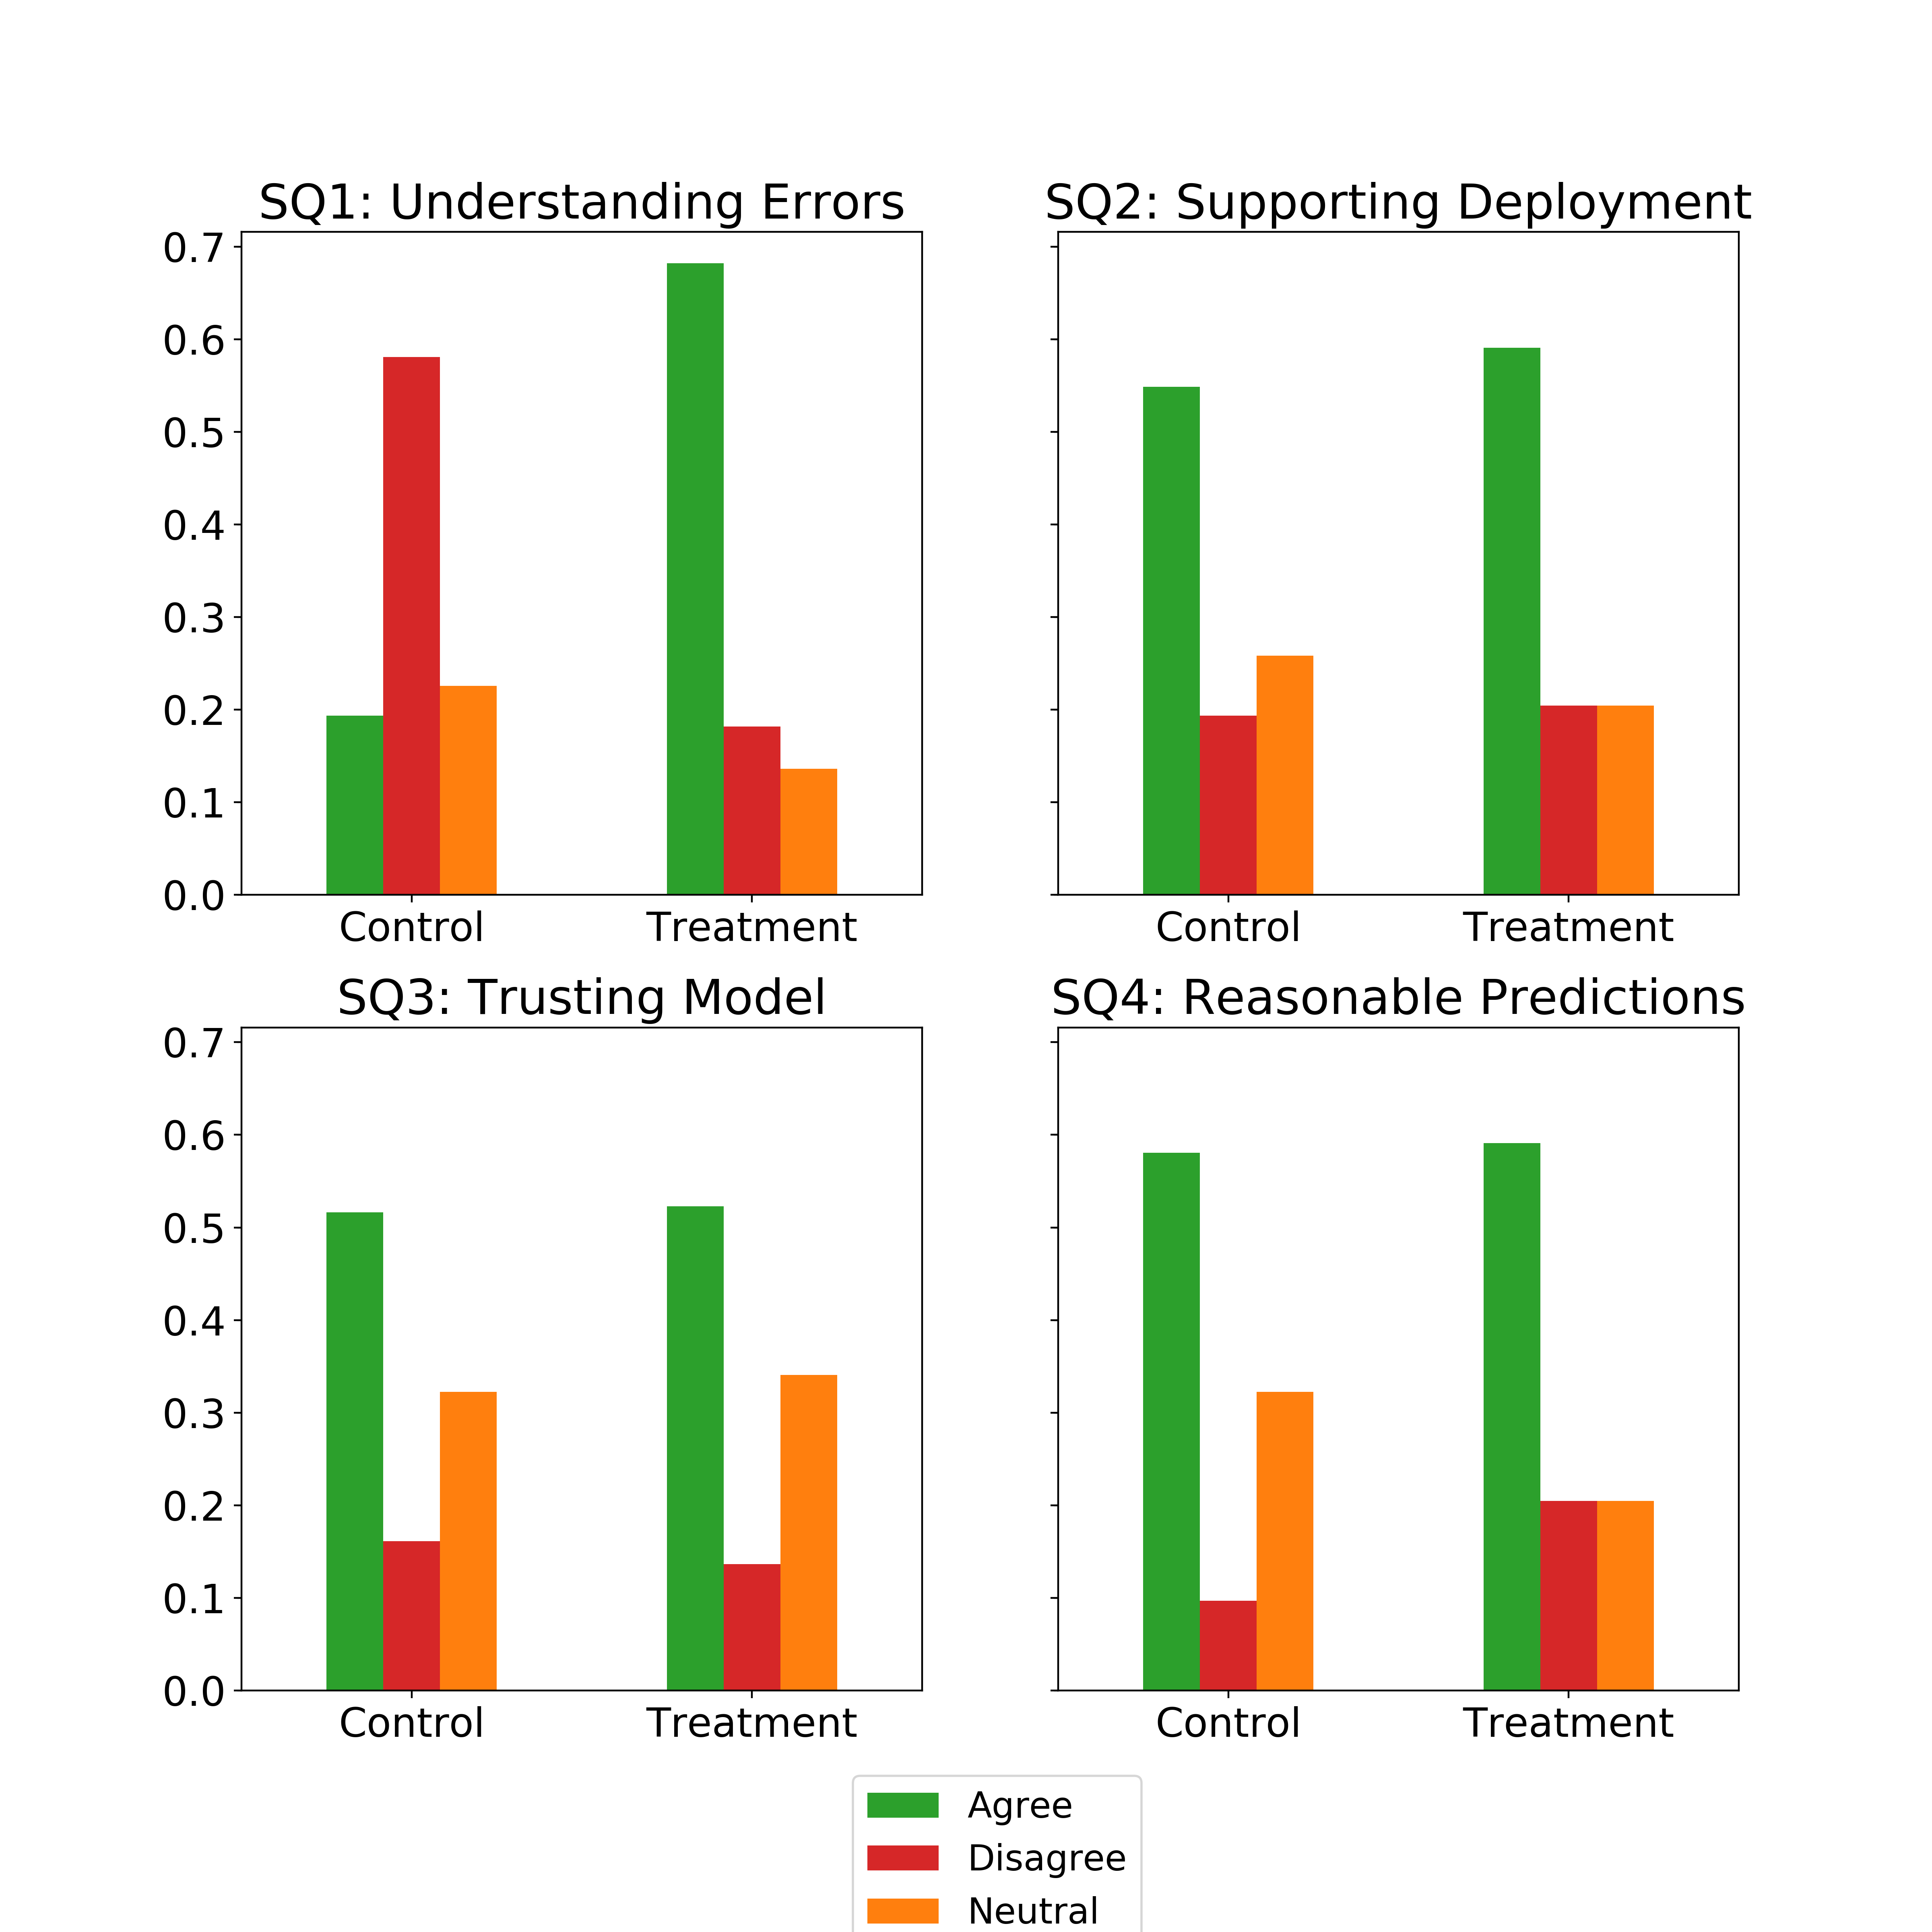
\includegraphics[clip,trim=0mm 0mm 0mm 0mm,scale=0.35]{04-research-mcbrp/treat-vs-control}
  \caption{Results from a within-subject study comparing answers between the treatment (\OurMethod{} explanation) and control (no explanation) groups.}
 \label{fig:treat-vs-control}
\end{figure}

\subsection{Subjective Questions}
In order to understand the impact of \OurMethod{} explanations on users' attitudes towards the model, we ask them the following subjective questions:
\begin{itemize}
	\item \textbf{SQ1:} I understand why the model makes large errors in predictions.
	\item \textbf{SQ2:} I would support using this model as a forecasting tool.
	\item \textbf{SQ3:} I trust this model.
	\item \textbf{SQ4:} In my opinion, this model produces mostly reasonable outputs.
\end{itemize}



To ensure our populations did not have different initial attitudes towards the model, we compared their answers on the subjective questions after only showing a visual description of the model. 
The visual description is a graph comparing the predicted sales to the actual sales, which allows users to see the distribution of errors made by the model (see Figure~\ref{fig:pred}). 
We found no statistically significant difference ($\chi^{2}$ test, $\alpha = 0.05$) in initial attitudes towards the model, which allows us to postulate that any difference discovered between the two groups is a result of the treatment they were given (i.e., \OurMethod{} explanation vs. no explanation). 

Figure~\ref{fig:treat-vs-control} shows the distributions of answers to the four subjective questions in the treatment and control groups. 
The difference in distributions is significant for SQ1 ($\chi^{2} = 18.2$, $\alpha = 0.0001$): users in the treatment group agree with the statement more than users in the control group. 
However, we find no statistically significant difference between the two groups for the remaining questions ($\chi^{2}$ test, $\alpha = 0.05$). 
That is, \OurMethod{} explanations help users understand why the model makes large errors in predictions, but do not have an impact on users' trust or confidence in the model, or on their willingness to support its deployment. 

\begin{table}[b]
\caption{Distribution of practitioners and researchers in the treatment and control groups.}
\label{table:background}
\centering
\begin{tabular}{lcc}
\toprule
\textbf{Background} & \textbf{Practitioners} & \textbf{Researchers} \\ 
\midrule
Treatment           & 52\%                   & 48\%                 \\
Control             & 58\%                   & 42\%                 \\ 
\bottomrule
\end{tabular}
\end{table}
